\chapter{LACC-M协议设计}
LACC-M(Load Adaptive CSMA/CA for Mobile underwater acoustic network) 协议是根据用水声网络进行数据采集的需求,针对有移动节点接入的单跳网络场景设计的协议。协议的基本流程参照了802.11协议,采用了CSMA/CA机制并用二进制退避算法计算随机退避的时间。在此基础上,考虑到移动节点的接入,加入了BCT帧以通知固定节点开始发送数据。同时,协议改进了数据帧重传机制,并且加入了自适应负载的数据帧发送机制来提高指定场景下的网络性能。

\section {基本原理介绍}
\subsection{冲突避免模式}
冲突避免是通过RTS/CTS握手机制实现的。RTS/CTS机制通过控制包预约信道来减少数据包碰撞,即用短包的碰撞代替长数据包的碰撞。发送节点准备发送数据时,首先侦听DIFS时间,如果信道空闲则开始发送RTS帧预约信道。RTS帧中包括了源节点地址,目标节点地址和本次通讯需要的最大持续时间。目标节点接收到RTS后,侦听SIFS时间后发送CTS帧进行响应。CTS帧中同样包括了源节点地址,目标节点地址和本次通讯需要的最大持续时间。非目标节点的其他节点在接收到RTS、CTS帧后,按照最大持续时间设置网络分配矢量(Network Allocation Vector, NAV)进行退避。源节点接收到CTS后,侦听SIFS时间后发送DATA帧。目标节点接收到数据包后,侦听SIFS时间后发送ACK包响应。其他节点接收到ACK帧后停止退避。
\begin{figure}[ht]
	\centering
	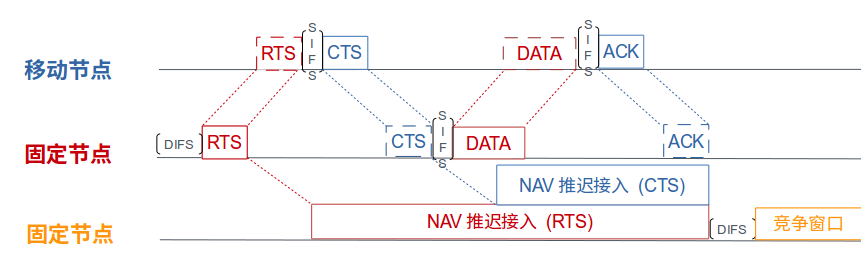
\includegraphics[scale=0.4]{figures/rtscts.png}
	\caption{
		RTS/CTS工作模式
	}
	\label{fig:example}
\end{figure}
\subsection{二进制指数退避算法}
在二进制指数退避算法\cite{赵占伟2011水声通信网络}中,当一个节点要向信道发送数据时,首先侦听信道状态,若信道空闲且空闲时间达到一个DIFS时,节点立即进行数据发送,否则,即节点侦听到信道状态为“忙”,此时节点会一直侦听下去,直至侦听到节点空闲一段DIFS时间后,根据退避算法产生一个退避时间值存入退避计时器,如果此时退避计时器里面已经有了退避时间值,那么就不将新产生的退避时间值存入退避计时器,然后进行退避,以避免和其它节点发生冲突。退避时间值是退避时隙(Slot Time)的整数倍,退避时隙是按物理层特性产生的值。节点在选好退避时间值后,如果信道在其退避期间一直空闲,那么节点会在一个完整的退避时隙后将退避时隙数减1,如果信道一直空闲到退避时隙数减到0时,节点就发送数据,否则,退避过程中又侦听到“忙”,则冻结退避计时器,停止退避,直至再次侦听到一段DIFS时间信道空闲后,再次启动退避计数器进行退避(退避时间值从上次退避后的值开始计算)。
\begin{figure}[ht]
	\centering
	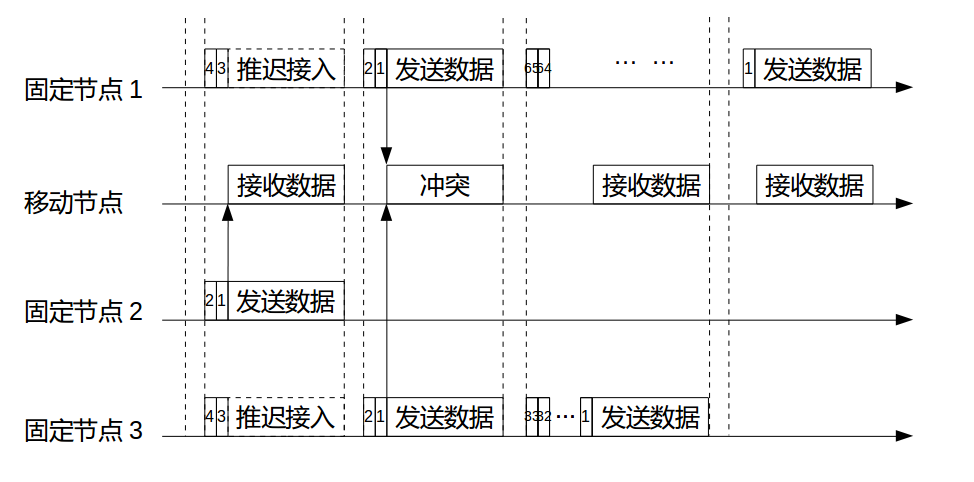
\includegraphics[scale=0.4]{figures/backoff.png}
	\caption{
		二进制指数退避流程
	}
	\label{fig5}
\end{figure}

退避时隙数在$[0,CW^i-1]$之间选择,$CW^i$是第$i$次退避时竞争窗口的大小,退避次数$i$由重传次数决定。节点首次向信道传输数据时,竞争窗口为$CW_min=CW^0-1$,$CW_min$是最小竞争窗口,$CW_max$是最大竞争窗口。$CW^i$的计算方法为
\begin{equation}
CW^i=2^i(CW^{i-1}+1)-1\ \ \ \  \ i=0,1,2,...,n
\end{equation}
当节点首次接入信道发送数据时,其竞争窗口值$CW_min$,第一次发送冲突后,竞争窗口值变为$CW_2$。直到到达最大竞争窗口值$CW_max$,下一次冲突后竞争窗口变为$CW_min$,重新开始循环。
退避时间(BackOffTime)的计算方式如下:
\begin{equation}
BackoffTime = Random \times SlotTime
\end{equation}
其中Random是在$[0,CW^i-1]$选择的时隙数,SlotTime指时隙时间。

\subsection{时隙和帧间间隔}
时隙(SlotTime)是指的一个时间片段,节点竞争接入信道之前需要经过相应的随机退避过程,退避过程就是由很多个时隙所组成的。参考802.11协议\cite{bianchi2000performance},时隙定义为
\begin{equation}
\begin{aligned}
SlotTime=&CCATime\mbox{(信道监测时间)}+Rx\mbox{(发送接收)}+TxTurnaround\\&Time\mbox{(转换时间)}+PropagationTime\mbox{(传播延迟)}+MAC\\&ProcessingDelay\mbox{(MAC层处理延迟)}
\end{aligned}
\end{equation}

短帧间间隔SIFS(Short Interfram Space)是最短的时间区段,用来间隔一次对话中的帧,如响应帧(CTS/ACK)和相邻的DATA帧等。在帧交换的两次传输之间使用最短间隔,可以防止其它正在等待信道的节点试图使用信道。参考802.11协议,SIFS定义为
\begin{equation}
\begin{aligned}
SIFSTime=&RXRFDelay\mbox{(发送延迟)}+RXPLCPDelay\mbox{(物理层头部接收}\\&\mbox{延迟)}+MACProcessingDelay\mbox{(MAC层处理延迟)}+ RxTx\\&TurnaroundTime\mbox{(发送接收转换时间)}
\end{aligned}
\end{equation}

分布协调功能帧间间隔DIFS(DCF Interframe Space)用于节点开始发送数据之前监测信道否空闲。如果信道已经空闲,则节点仍需等待DIFS段时间才开始发送数据;而如果在DIFS时间段内任一时刻信道被监测为忙,则节点不得不推迟它的数据发送。DIFS定义为
\begin{equation}
DIFS=SIFS+(2*SlotTime)
\end{equation}

在水声信道环境中,由于传播时延导致时隙时间过长,进而导致DIFS和随机退避时间过长,即数据传输时空闲时间过长,影响了协议的整体性能。减小时隙时间可以减小空闲时间占比,但同时也会带来包冲突概率的增加。综合这两方面的影响,最后将时隙时间设定为1s,SIFS设定为0.5s。
\section {移动节点接入离开机制}
通过引入BCT帧控制移动节点的接入和离开,其中包括了源节点地址,目标节点地址和网络负载情况。移动节点以$1/T_{interval}$速率定时发送广播包BCT,开始向最近的移动节点发送CBR数据流。如果固定节点在$2*T_{interval}$时间内没有接收到广播包,则停止发送CBR数据流。机制流程见图\ref{fig6}。其中,CBR数据流是以确定的速率产生通信量,分组尺寸固定,可在分组间隔之间产生随机抖动。
\begin{figure}[!ht]
	\centering
	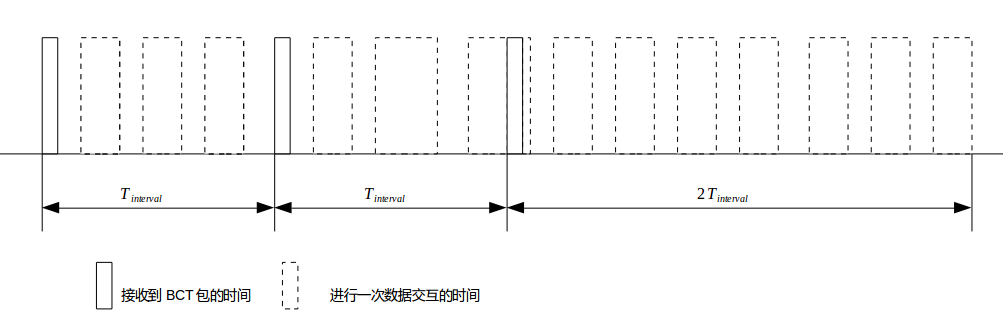
\includegraphics[scale=0.4]{figures/mj.png}
	\caption{
		移动节点接入离开机制
	}
	\label{fig6}
\end{figure}

BCT帧的发送接收不影响正在进行的一轮传输。例如在发送节点接收到CTS还未发送DATA帧时接收到了BCT帧,发送节点的状态仍为CTS,在接收完BCT帧后,继续发送DATA帧。

固定节点接收到BCT帧后,将移动节点的信息存在HASH表中移动节点的地址作为key值,移动节点与固定节点的距离等信息存在一个struct中作为value值。固定节点准备发送数据时,将HASH表内的节点信息进行排序,选择距离最近的节点发送数据。

\section {数据帧重传机制}
考虑到减小时隙时间导致载波侦听时间不够充分,包冲突概率增加,以及BCT帧的引入带来的包冲突可能性这两个方面,加入了数据包重传机制。在802.11协议中,源节点发送了DATA包但没有收到ACK确认帧的情况下,会在发送函数定时器超时后重新开始一轮新的数据传输,经过退避时间和DIFS时间倒计时后再发送RTS帧。这个重传流程在包冲突概率较大的情况下开销过大,影响传输性能。

因此,在发送DATA帧超时后立即重传DATA帧是一个可行的解决方法。同时,需要修改其他节点的推迟接入时间,在原推迟时间的基础上加上timeout(DATA包一次发送超时时间)、SIFS、txtime(传输时间)和MaxPropagationDelay(最大传播时延)。

\begin{figure}[!ht]
	\centering
	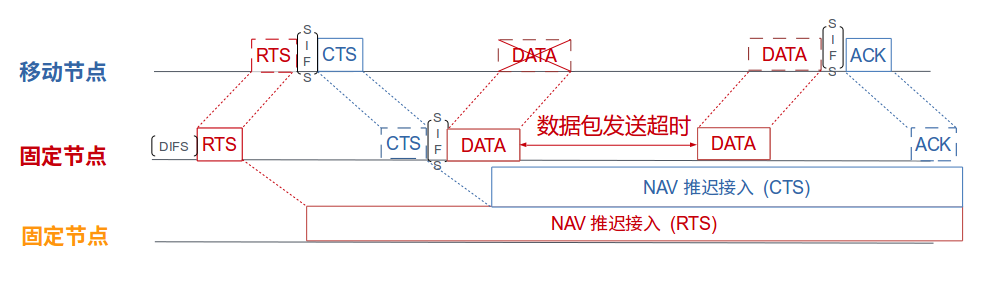
\includegraphics[scale=0.4]{figures/chongchuan.png}
	\caption{
	     一次传输超时情况下的数据帧重传流程
	}
	\label{fig:example}
\end{figure}

\section {自适应负载变化的数据帧发送机制}
网络负载较大时,数据包的RTS/CTS握手机制带来的控制开销较大,对于不同的网络负载情形,可以采用不同的数据包传输机制。在高负载的情况下,发送节点可以在一次RTS/CTS握手后发送两个DATA帧,两个DATA包间间隔SIFS,接收节点在接收到第二个DATA包后发送ACK信号。低负载的情况下,仍然采用原来的流程。

由于数据包传输机制的改变,节点的推迟接入时间和发送超时时间会有不同。可以通过在BCT帧中增加一位数据位标志网络的负载情况,固定节点在接收到BCT广播帧后更改自己的数据传输模式。
\begin{figure}[!ht]
	\centering
	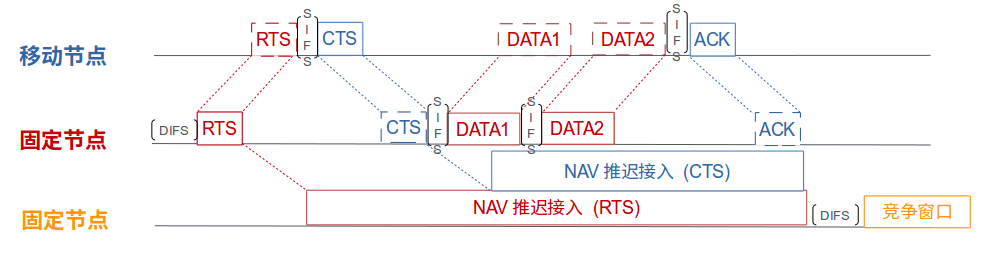
\includegraphics[scale=0.4]{figures/highload.png}
	\caption{
		高负载情况下的数据帧传输流程
	}
	\label{fig:example}
\end{figure}



\endinput